\documentclass[12pt]{article}

\usepackage{graphicx}
\usepackage{epstopdf}
\usepackage[english]{babel}
\usepackage[latin5]{inputenc}
\usepackage{hyperref}
\usepackage[left=3cm,top=3cm,right=3cm,nohead,nofoot]{geometry}
\usepackage{datenumber}

\begin{document}

\begin{center}
\Huge
Project: Enigma Machine and Turing-Welchman Bombe

\vspace{10mm}
\Large
Maria Camila REMOLINA GUTI�RREZ
\large
maria.remolina\_gutierrez@telecom-sudparis.eu

\vspace{5mm}
\Large
Advisor: Prof. Eric RENAULT

\vspace{5mm}
\normalsize
\today
\end{center}

\vspace{5mm}
\begin{abstract}
	This is the work proposal to follow in the course Project as part of the master M1 in Computer Science and Communication Networks at T�l�com SudParis. The goal is to implement the Enigma machine used in World War II, followed by the Bombe machine that breaks the cipher, created by Alan Turing and Gordon Welchman at Bletchley Park.
\end{abstract}

\section{Introduction}

The enigma machine is a cipher machine used by the Nazi Germany during World War II in order to send secret coded messages. It was initially a commercial machine bought by banks are businesses. But then the military took it and added an extra security layer called plugboard. It was innovative at the time because it was not a substitution cipher, i.e. the same letter can get different results after encryption. \\

The machine works by a combination of moving rotors and inside wiring as seen in Fig. {fig:machine}. The way to use it is that when the sender types a message, a bulb lights up indicating the correspondent coded letter. Then, in order to decode, the receiver types the coded message he received and the initial message lights up on the board. In war times the coded messages were transmitted over morse code. \\

\begin{figure}[h!]
	\centering
	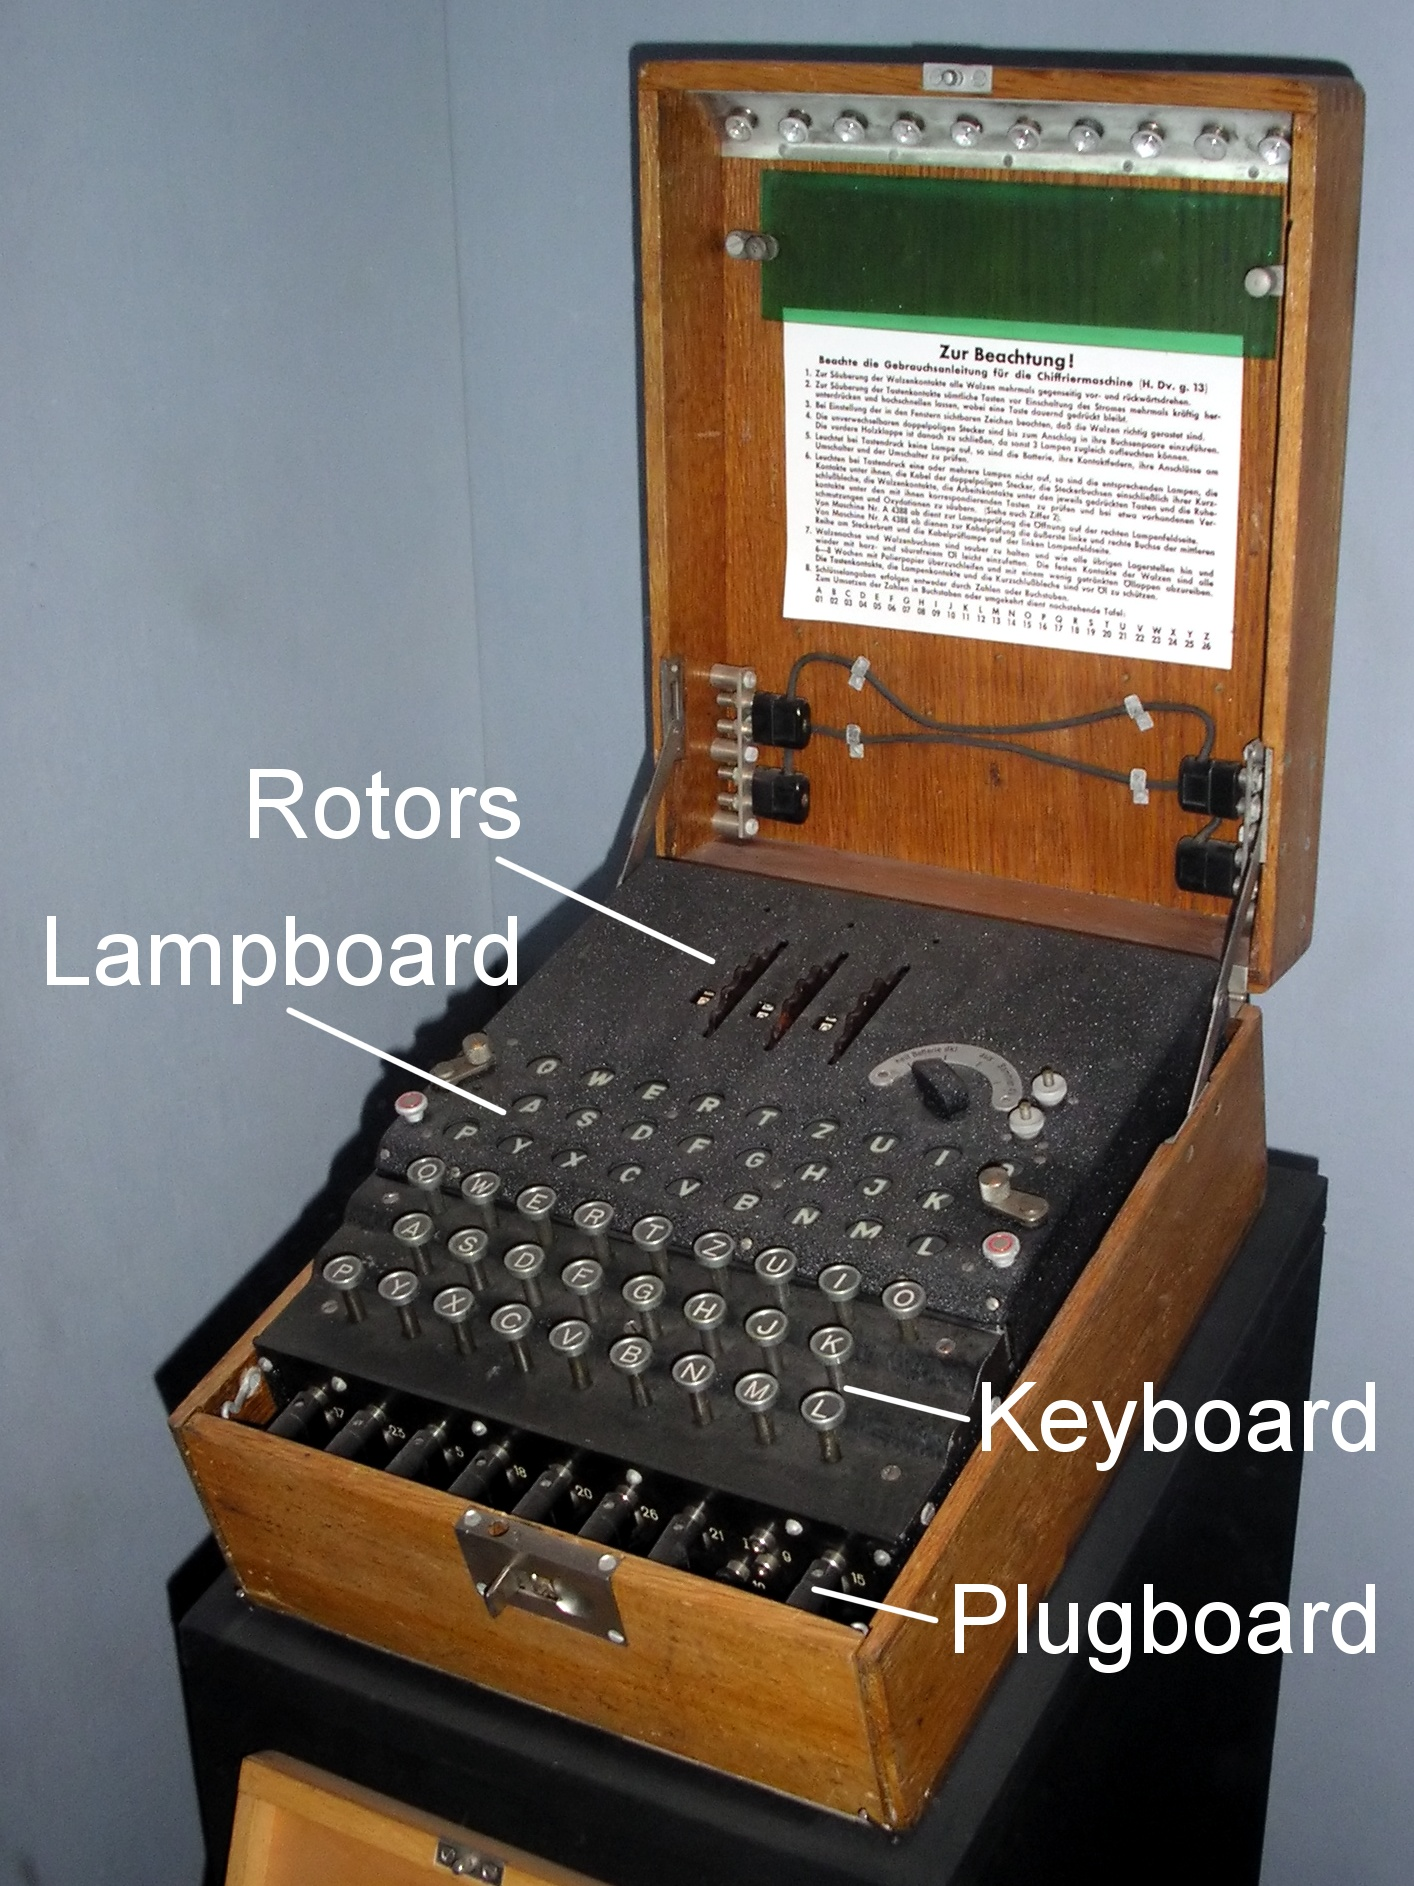
\includegraphics[width=\textwidth]{img/machine}
	\caption{Enigma Machine - Military Edition}
	\label{fig:machine}
\end{figure}

In the military version of the Enigma Machine there were 5 possible rotors to pick from, each with 26 possible positions, then there were 10 possible switching in the plugboard that could choose a pair from the available 26 letters. That accounts for $158962555217826360000$ different combinations for
the setting of the army Enigma Machine \cite{numberphile1}. The initial setting for each day was given to the bases in a sheet of paper that had the monthly configurations of the machine. So they changed the setting everyday. \\

So in order to decipher the code, you needed either to have the code sheet or to break the message. This latter was what the scientists at Bletchley Park did; and what I will try to recreate in this project. 

\section{General Goal}

To understand the code breaking process behind the enigma cipher.


\section{Specific Goals}

\begin{itemize}
	\item To implement the Enigma machine with software
	\item To implement the Bombe machine that breaks the Enigma cipher
	\item To understand the mathematical and probabilistic techniques used to break a cipher with limited time and computational resources. 
	\item To understand the weaknesses exploited that allowed to break the Enigma cipher
\end{itemize}


\section{Methodology}

I will create 2 different programs within the same project: 

\begin{enumerate}
	\item The Enigma machine 
	\item The Bombe machine
\end{enumerate}

The implementation of both will be in Python and it will be publicly available in the GitHub repository \url{https://github.com/mariacamilarg/enigma_bombe}. As for the computational resources, I will need only my personal computer (with Linux O.S.) with standard architecture.


\section{Work Schedule}

This will be the main work of the course Scientific Project with 2.5 ECTS. It will be performed during the course of 2 months approximately, in the time stipulated for the class. The delivery date will be in mid June of 2019.


\begin{thebibliography}{10}

% https://www.youtube.com/watch?v=G2_Q9FoD-oQ
\bibitem{numberphile1} Numberphile. \textit{158,962,555,217,826,360,000 (Enigma Machine)}. YouTube (2013).

\bibitem{hodges} A. Hodges. \textit{Alan Turing: The Enigma}. Princeton, N.J: Princeton University Press (2012). 

\end{thebibliography}

\vspace{2cm}
\section*{Advisor Signature}

\vspace{2cm}
\section*{Student Signature}

\end{document} 